% !TeX root = thesis.tex

\chapter{Models for uncertainty aware object detection}\label{ch:models-for-uncertainty-aware-object-detection}
In this chapter, we will discuss the different uncertainty-aware models introduced in \cref{ch:literature-study_section:uncertainty-aware-ai-models} and compare their ability to capture and communicate uncertainty.
We will first discuss the way an uncertainty-aware model is trained and evaluated, after which we will discuss the different models in more detail, ending with a comparison of the different models for our use case.

\section{The structure of an uncertainty aware model}\label{ch:models-for-uncertainty-aware-object-detection_section:the-structure-of-an-uncertainty-aware-model}
An uncertainty-aware model differs from a normal model, in the sense that it needs to output its uncertainty alongside the prediction.

The model outputs a number of values, depending on what the application requires:
If we want our model to output a single value, for example predicting the time it takes for a robot to move to a certain point, in a conventional model, it would output a value in seconds, for example 5.2 seconds.
However, in an uncertainty aware model, it would output two values, for example 5.2 seconds and 0.8 seconds.
The first value is the prediction, and the second value is the uncertainty of that prediction.
In our case, we want to predict the position of an object in 2D space, so we want to output the x and y coordinates of the object, along with the uncertainty of those predictions.
This means that our model will output four values, for example 57.2, 33.4, 0.8, 0.6.
The first two values are the predicted x and y coordinates, and the last two values are the uncertainty of those predictions.

The way of computing the uncertainty of a prediction depends on the kind of uncertainty we want to cover.

For aleatoric uncertainty, the uncertainty linked to the data, we can use a single model with two outputs.
The model will learn the distribution of training data and, when trained properly, will be able to tell when something is off.
In practice, we train a model with two outputs (one extra for every predicted value) the conventional way with a loss function and back-propagation.
How this is done in detail, will be discussed in~\cref{ch:models-for-uncertainty-aware-object-detection_section:training-evaluation}.

Epistemic uncertainty, the uncertainty associated with the model parameters, is a bit more complex as it requires multiple models to capture the uncertainty.
The idea of communicating the uncertainty in practice, is very related to aleatoric uncertainty, as it also outputs two values (one extra per predicted value), one prediction and an uncertainty value.
However, the uncertainty value is no longer a value that the individual models need to learn, rather it is the ``agreement or disagreement'' between the models.
This ``agreement or disagreement'' can be interpreted in different ways depending on the application of the model.
For regression tasks, the most obvious choice is the variance of the predictions, but it can also be an interval in which the predictions fall, or even a distribution where the user can ask for a specific confidence level.
For classification tasks, the most obvious choice is the entropy of the predictions, but it can also be the variance of the predicted probabilities.

The nice thing about the way uncertainty aware models are structured, is the fact that this is exactly the same for both aleatoric and epistemic uncertainty.
A single model, which can only capture aleatoric uncertainty, will output a value for the prediction along with a value for the uncertainty.
Multiple ``standard'' (non-uncertainty aware) models combine for an ensemble of models which can capture epistemic uncertainty.
This will also output a value for the prediction along with a value for the uncertainty.
Both these uncertainties can be captured in a single model by using an ensemble of models capable of capturing aleatoric uncertainty (see \cref{ch:literature-study_section:uncertainty-aware-ai-models_subsection:deep-ensemble-methods_paragraph:ensembling}); this way we can capture both the uncertainty linked to the data and the uncertainty linked to the model parameters.

\section{Training and evaluating uncertainty aware models}\label{ch:models-for-uncertainty-aware-object-detection_section:training-evaluation}
Training an uncertainty-aware model differs quite a bit from training a conventional \gls{nn}.
This is because of the nature of the models, as they need to communicate uncertainty along with the prediction.
We thus need a way to train the model to include uncertainty in its predictions, and we also need a way to evaluate the model on its ability to capture and communicate uncertainty.
There are a few ``new'' ways of thinking about when a model is doing what it is supposed to do, and when it is not:
\begin{itemize}
    \item If the model is sure about its prediction, and the prediction is correct, great! The model is doing its job.
    \item If the model is sure about its prediction, but the prediction is wrong, then the model is not doing its job as it is unable to communicate its faults.
    \item If the model is unsure about its prediction, and the prediction is wrong, then the model is doing its job as it is able to communicate its uncertainty about its prediction.
    \item If the model is unsure about its prediction, but the prediction is correct, then the model is not doing its job as it is unable to communicate its confidence in its prediction.
\end{itemize}
We need a way so these cases can be captured in a loss function, so that the model can learn to do what it is supposed to do.
Fortunately, there already exists such a loss function, Gaussian \gls{nll} loss~\cite{src:deep-ensemble-methods} (\cref{eq:gaussian-nll-loss}).

\begin{equation}\label{eq:gaussian-nll-loss}
    \mathcal{L} = -log(p_\theta(\mathbf{y}_n|\mathbf{x}_n)) = \frac{log(\bm{\sigma}^2_\theta(\mathbf{x}_n))}{2} + \frac{(\mathbf{y}_n-\bm{\mu}_\theta(\mathbf{x}_n))^2}{2\bm{\sigma}^2_\theta(\mathbf{x}_n)} + constant
\end{equation}

Where $\bm{\mu}_\theta(\mathbf{x}_n)$ are the predicted means, $\bm{\sigma}^2_\theta(\mathbf{x}_n)$ are the predicted variances, and $\mathbf{y}_n$ are the true values.
In our case, $\mathbf{y}_n$ is a 2D vector containing the true x and y coordinates of the object, $\bm{\mu}_\theta(\mathbf{x}_n)$ and $\bm{\sigma}^2_\theta(\mathbf{x}_n)$ are also 2D vectors containing the predicted x and y coordinates and the predicted variance, respectively.
These vectors do not change anything fundamental to the loss function.

This loss function captures the cases we discussed above, as it penalizes the model for being sure about a wrong prediction, and it also penalizes the model for being unsure about a correct prediction.
Even more, it optimizes the model in such a way that the predicted uncertainty ($\sqrt{\sigma^2_\theta(\bm{x})}$) is exactly equal to the error of the mean prediction ($\sqrt{(\mu(\bm{x}) - y)^2}$).
This can be proven by taking the derivative of the loss function with respect to the variance and setting it to zero (\cref{eq:loss-function-derivative}).

\begin{equation}\label{eq:loss-function-derivative}
    \begin{aligned}
        &\frac{\partial \mathcal{L}(\theta)}{\partial \sigma^2_\theta} = 0 \\
        \iff& \frac{\partial}{\partial \sigma^2_\theta} \left( \frac{\log(\sigma^2_\theta)}{2} + \frac{(y-\mu_\theta)^2}{2\sigma^2_\theta} + \text{constant} \right) = 0 \\
        \iff& \frac{1}{2\sigma^2_\theta} - \frac{(y-\mu_\theta)^2}{2\sigma^4_\theta} = 0 \\
        \iff& \frac{1}{2\sigma^4_\theta} \left( \sigma^2_\theta - (y-\mu_\theta)^2 \right) = 0 \\
        \iff& \sigma^2_\theta - (y-\mu_\theta)^2 = 0 \\
        \iff& \sigma^2_\theta = (y-\mu_\theta)^2 \\
        \iff& \sqrt{\sigma^2_\theta} = \sqrt{(y-\mu_\theta)^2}
    \end{aligned}
\end{equation}

\cref{eq:loss-function-derivative} shows how the loss optimizes a single model (not an ensemble) with a single output (mean and variance).
This logic can, however, easily be extended to ensembles as well as models with multiple outputs.
Ensembles also output a mean and a variance, only the meaning of the variance is different, as it captures the epistemic uncertainty instead of the aleatoric uncertainty (or both if the base models are uncertainty-aware).
Multiple outputs are also not a problem, as the loss function can be applied to each output separately, and the total loss is just the mean of the losses of each output.

\section{Data scaling}\label{ch:models-for-uncertainty-aware-object-detection_section:data-scaling}
During the training of the models below, we came across an issue related to the data.
More specifically, the mismatching of the data's order of magnitude and the model's weights' order of magnitude.
The data we gathered is in mm, so the values of the $x$ and $y$ coordinates are fairly big hovering between 10 and 500.
The weights of the model, on the other hand, are initialized with small values, between 0 and 1, and during the training, they do not change much in terms of order of magnitude.
This means that the model needs to somehow find a way to scale to match the order of magnitude of the outputs, which is very challenging.

To solve this issue, we started by scaling the outputs of the model by a $10^{-3}$ factor, so the model's outputs are somewhat in the same order of magnitude as the model's weights.
This helped a lot, but is not the most elegant solution, as this factor is arbitrarily chosen and is not based on any theoretical foundation.

A more elegant way to calculate this factor is to use the data itself.
We can calculate the mean and standard deviation of the $x$ and $y$ coordinates in the training data, and use these to normalize the data.
The scaling factor can be calculated as \cref{eq:scaling-factor}, which centers the data to have a zero mean and unit variance.
Again, note the vectors in the equation, as we have two values for the $x$ and $y$ coordinates.

\begin{equation}\label{eq:scaling-factor}
    \mathbf{z} = \frac{\mathbf{y} - \bm{\mu}}{\bm{\sigma}}
\end{equation}

This way, the model's outputs are in the same order of magnitude as the model's weights, and the model can learn to predict values that are in the same order of magnitude as the data.
After the forward pass of the model, we can then unscale the outputs using \cref{eq:unscale-factor} to get the actual predictions in mm.

\begin{equation}\label{eq:unscale-factor}
    \mathbf{y} = \mathbf{z} \cdot \bm{\sigma} + \bm{\mu}
\end{equation}

\section{Deep ensembles}\label{ch:models-for-uncertainty-aware-object-detection_section:deep-ensembles}
A deep ensemble, as explained in \cref{ch:literature-study_section:uncertainty-aware-ai-models_subsection:deep-ensemble-methods}, is an ensemble of \glspl{dnn}.
We explored two kinds of deep architectures: a custom \gls{cnn} and ResNet-18~\cite{src:resnet}, both with and without pretrained weights.

The training loop we used is very similar to the approach described in \cref{ch:literature-study_section:uncertainty-aware-ai-models_subsection:deep-ensemble-methods}.
Training each model on its own, then combining them to be an ensemble.

The architecture of the models was kept the same for all the models in the ensemble, the initialization of the model's weights was varied as well as the way the training examples were fed to the models.
By differing the initialization of the model's weights and the shuffling of training examples, the models in the ensemble are different enough to obtain a good result~\cite{src:deep-ensemble-methods}.
This means bagging is not needed, however, it is implemented, so it can be easily turned on if needed.

During training, adversarial examples were generated using the \gls{fgsm}.
Each input batch was perturbed in the direction of the loss gradient's sign.
This creates adversarial samples that are perceptually identical to the originals, yet mathematically optimized to maximize the model's prediction error.
The loss function we used is the one described in \cref{ch:models-for-uncertainty-aware-object-detection_section:training-evaluation}.
After each epoch, the models were evaluated on the validation set, and the best model was saved.
This way, the best model we got during training is saved and used in the ensemble, rather than the last model we got after training, which might not be the best one due to, for example, overfitting.
The training script also schedules the learning rate, so it is reduced after 10 epochs without improvement on the validation loss, this is a way it so the model is finetuned well.
We mostly trained 5 models for each ensemble, as suggested by the paper~\cite{src:deep-ensemble-methods}, but this could also easily be changed.

For our own convenience, we created a configuration file to easily change the architecture of the models, the way the training examples are fed to the models, some hyperparameters, etc.

\subsection{Simple \gls{cnn}}\label{ch:models-for-uncertainty-aware-object-detection_section:deep-ensembles_subsection:simple-cnn}
For our custom \gls{cnn}, we used an architecture which is easily changeable, so we can easily add or remove layers to see the effect on the performance of the model.
Generally, the architecture consists of a few ``convolutional blocks'' followed by a single fully connected layer.
A ``convolutional block'' consists of a convolutional layer, followed by a ReLU activation function and a max pooling layer.
The kernel size and padding of the convolutional layers are kept constant at 5 and 2 respectively, as are the kernel size of 2 and a stride of 2 for the max pooling layers.
The number of channels of the convolutional layers and the number of convolutional blocks can be easily changed in the configuration file.

The first convolutional layer's input channels are fixed at 3 or 4, depending on the input data to include the depth channel or not, while its output channels can be changed.
The fully connected layer's output channels are also fixed at 4, two for the predicted x and y coordinates, and two for the predicted variance of those coordinates.

As an example, consider an architecture with three ``convolutional blocks'', the first one with 8 output channels, the second one with 32, and the third one with 64.
After the ``convolutional blocks'', the output is flattened and fed to a fully connected layer with 4 output channels.

\paragraph{Comparing architectures and hyperparameter tuning}\label{ch:models-for-uncertainty-aware-object-detection_section:deep-ensembles_subsection:simple-cnn_comparing-architectures-and-hyperparameter-tuning}
We tested a lot of different combinations of architectures and hyperparameters.
We compared them using the validation loss on the full ensemble as well as the individual models' training and validation loss curves.
\cref{tab:simple-cnn-architectures-comparison} and \cref{fig:cnn-loss-curves} show the results of some of the architectures we tested.

\begin{table}[ht]
    \centering
    \begin{tabular}{c !{\vrule width 2pt} c|c|c|c|c|c !{\vrule width 2pt} c}
        \textbf{Index} & \textbf{Architecture} & \textbf{Lr} & \textbf{Bs} & \textbf{Br} & \textbf{Epochs} & \textbf{m} & \textbf{Loss} \\
        \hline
        1 & [8, 16, 32] & $5\cdot10^{-4}$ & 32 & None & 60 & 5 & -2.9775 \\
        2 & [8, 16, 32] & $1\cdot10^{-3}$ & 32 & None & 60 & 5 & -2.1718 \\
        3 & [16, 32, 64] & $5\cdot10^{-4}$ & 32 & None & 60 & 5 & -2.6241 \\
        4 & [8, 16, 32] & $5\cdot10^{-4}$ & 16 & None & 60 & 5 & -2.8678 \\
        5 & [8, 16, 32] & $5\cdot10^{-4}$ & 32 & 0.8 & 60 & 5 & -2.3003 \\
        6 & [8, 16, 32] & $5\cdot10^{-4}$ & 32 & None & 60 & 3 & -2.9813 \\
    \end{tabular}
    \caption[Comparison of different architectures for the simple CNN model]{
        Comparison of different architectures for the simple CNN model.
        ``Lr'' stands for learning rate, ``Bs'' stands for batch size, ``Br'' stands for bagging ratio, ``m'' stands for the number of models in the ensemble, and ``Loss'' stands for the ensemble validation loss.
    }
    \label{tab:simple-cnn-architectures-comparison}
\end{table}

\begin{figure}[]
    \centering
    \begin{subfigure}{0.49\textwidth}
        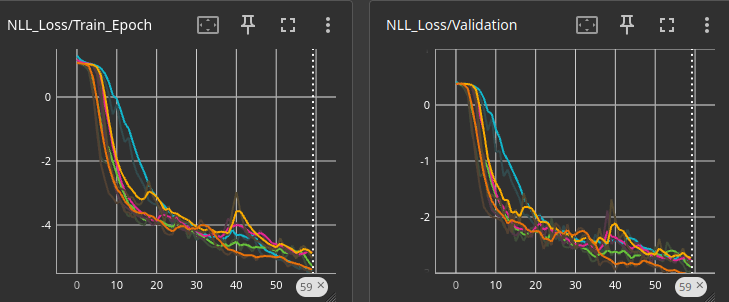
\includegraphics[width=\textwidth]{static/cnn/1-loss.png}
        \caption{Training and validation loss curves of the individual models of ensemble 1.}
        \label{fig:cnn-1-loss-curves}
    \end{subfigure}
    \begin{subfigure}{0.49\textwidth}
        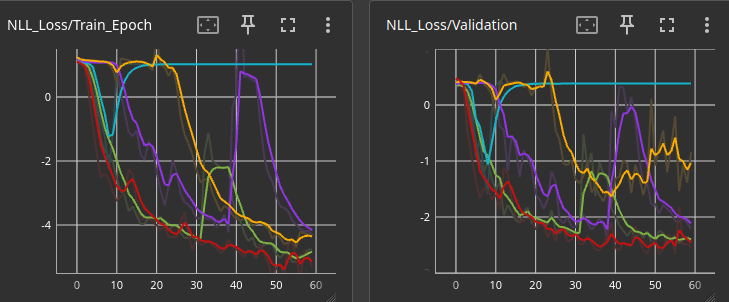
\includegraphics[width=\textwidth]{static/cnn/2-loss.png}
        \caption{Training and validation loss curves of the individual models of ensemble 2.}
        \label{fig:cnn-2-loss-curves}
    \end{subfigure}
    \begin{subfigure}{0.49\textwidth}
        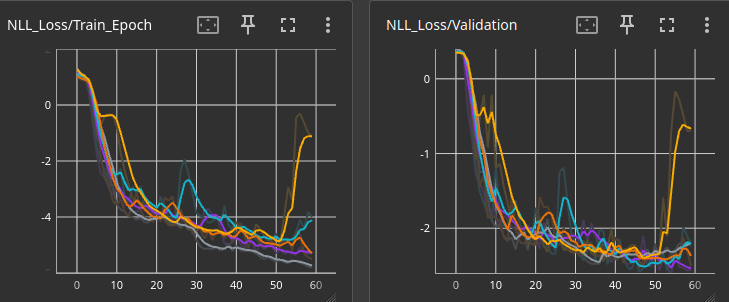
\includegraphics[width=\textwidth]{static/cnn/3-loss.png}
        \caption{Training and validation loss curves of the individual models of ensemble 3.}
        \label{fig:cnn-3-loss-curves}
    \end{subfigure}
    \begin{subfigure}{0.49\textwidth}
        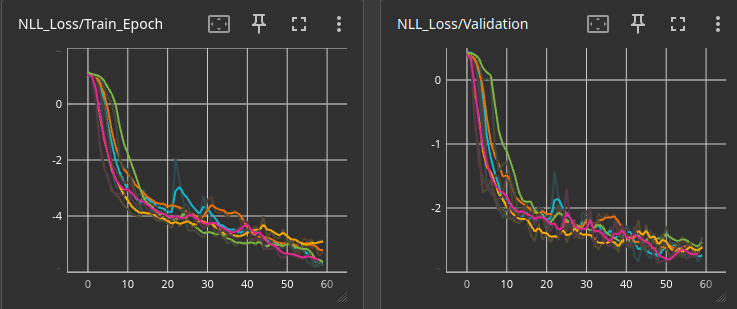
\includegraphics[width=\textwidth]{static/cnn/4-loss.png}
        \caption{Training and validation loss curves of the individual models of ensemble 4.}
        \label{fig:cnn-4-loss-curves}
    \end{subfigure}
    \begin{subfigure}{0.49\textwidth}
        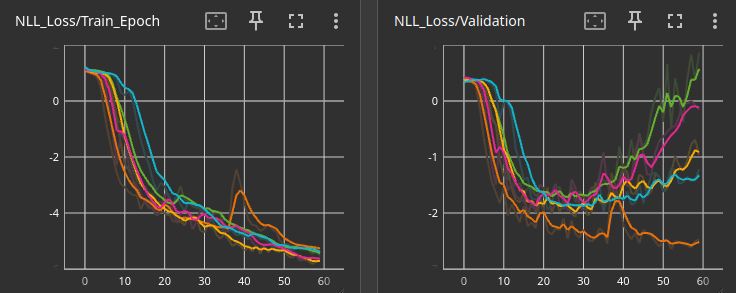
\includegraphics[width=\textwidth]{static/cnn/5-loss.png}
        \caption{Training and validation loss curves of the individual models of ensemble 5.}
        \label{fig:cnn-5-loss-curves}
    \end{subfigure}
    \begin{subfigure}{0.49\textwidth}
        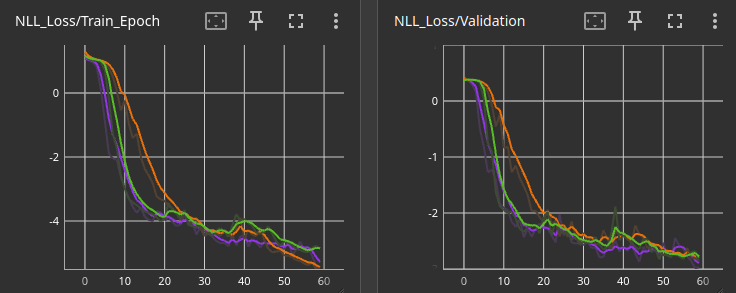
\includegraphics[width=\textwidth]{static/cnn/6-loss.png}
        \caption{Training and validation loss curves of the individual models of ensemble 6.}
        \label{fig:cnn-6-loss-curves}
    \end{subfigure}
    \caption{Training and validation loss curves of the individual models of the different custom \gls{cnn} ensembles.}
    \label{fig:cnn-loss-curves}
\end{figure}

When looking purely at the validation loss of the different models, we can see that the differences are quite small, except for the model with a learning rate of $1\cdot10^{-3}$ (model 2) and model 5 with bagging, which have a relatively high validation loss compared to the other models.
Model 2 is probably worse because the model was too aggressive in its learning, and thus was not able to find a good minimum and optimize properly.
This is also reflected in the training and validation loss curves of the individual models (\cref{fig:cnn-2-loss-curves}), as they are very unstable and do not show a clear downward trend.
Model 5 has less data to train on, as it is trained on only 80\% of the training data.
This is reflected in the loss curves (\cref{fig:cnn-5-loss-curves}), as the models seem to settle faster on a higher loss, after which they overfitted quite a bit.

When comparing the different architectures (model 1 vs model 3), we can see that the performance drops quite a bit.
The loss curves (\cref{fig:cnn-1-loss-curves} and \cref{fig:cnn-3-loss-curves}) show that the model 3 does not find a good minimum as easily as model 1.

Having 5 models in the ensemble was recommended by the paper~\cite{src:deep-ensemble-methods}, as it brings a nice balance between diversity and performance.
However, we found that a model with only 3 \gls{cnn} models in the ensemble (model 6) performed very similarly to one with 5 \glspl{cnn} in the ensemble.
This means that all the models in the ensemble have converged to a similar minimum despite the differences in initialization and training, and thus adding more models to the ensemble does not bring a significant change in performance.
3 models in the ensemble obviously reduces the size of the model and the inference time, so it is a good option if the performance is not significantly worse than with 5 models.

We will keep model 6 for further comparison with the other models, as it has the best performance while also being the smallest.

\subsection{ResNet\cite{src:resnet}}\label{ch:models-for-uncertainty-aware-object-detection_section:deep-ensembles_subsection:resnet}
ResNet~\cite{src:resnet} is a very popular architecture for image classification tasks, and it has been shown to perform well.
The main idea behind ResNet is the use of residual connections (shown in \cref{fig:residual-block}), which allow the model to learn residual functions instead of direct mappings.
This allows the model to learn more complex functions and to avoid the vanishing gradient problem, which is a common problem in deep learning.
The architecture of ResNet is based on a series of residual blocks, which consist of two or three convolutional layers with a skip connection between the input and the output of the block.
The number of residual blocks and the number of convolutional layers in each block can be varied to create different versions of ResNet, such as ResNet-18, ResNet-34, ResNet-50, etc.

\begin{figure}
    \centering
    
\includegraphics[width=0.5\textwidth]{residual-block.png}
    \caption{A residual block, the main building block of ResNet.}
    \label{fig:residual-block}
\end{figure}

The ResNet architecture we used for our experiments is a ResNet18, which is quite a small version of ResNet with 8 residual blocks.
The architecture, as originally designed, is used for image classification tasks, so we needed to modify it to be used for our regression task.
The main modification we made is to replace the final fully connected layer, which has 1000 output channels for the 1000 classes in ImageNet, with a fully connected layer with 4 output channels.
We made it possible to change the number of residual blocks used in the architecture, so we can easily test how the different layers react to our use case.
If we choose to, for example, only use the first 4 residual blocks, we take the first four residual blocks.

The PyTorch~\cite{src:pytorch} library provides a convenient implementation of ResNet, along with pretrained weights.
These are weights that have been trained on ImageNet-1K~\cite{src:imagenet}, a large dataset of images with 1000 classes.
Using pretrained weights can be beneficial for our task, as we do not need to train the full architecture's weights from our own dataset, which would be too small for training such a large architecture.
The pretrained weights can be used as a starting point for training our model, and we can fine-tune the model on our own dataset to adapt it to our specific task.

\paragraph{Comparing architectures and hyperparameter tuning}\label{ch:models-for-uncertainty-aware-object-detection_section:deep-ensembles_subsection:resnet_comparing-architectures-and-hyperparameter-tuning}
In \cref{tab:resnet-architectures-comparison}, we show the results of some of the architectures we tested for the ResNet model.
The hyperparameters were varied to obtain the best validation loss

\begin{table}[ht]
    \centering
    \begin{tabular}{c !{\vrule width 2pt} c|c|c|c|c|c|c !{\vrule width 2pt} c}
        \textbf{Index} & \textbf{Architecture} & \textbf{Lr} & \textbf{Bs} & \textbf{Br} & \textbf{Epochs} & \textbf{m} & \textbf{FB} & \textbf{Loss} \\
        \hline
        1 & 4 & $1\cdot10^{-4}$ & 32 & None & 100 & 5 & Yes & -2.1134 \\
        2 & 2 & $1\cdot10^{-4}$ & 32 & None & 100 & 5 & Yes & 0.9102 \\
        3 & 6 & $1\cdot10^{-4}$ & 32 & None & 100 & 5 & Yes & 1.7538 \\
        4 & 4 & $1\cdot10^{-3}$ & 32 & None & 100 & 5 & Yes & 1.7653 \\
        5 & 4 & $1\cdot10^{-4}$ & 16 & None & 100 & 5 & Yes & -2.1212 \\
        6 & 4 & $1\cdot10^{-4}$ & 32 & None & 100 & 3 & Yes & -2.1038 \\
        7 & 4 & $1\cdot10^{-4}$ & 32 & None & 100 & 5 & No & -2.2162 \\
        8 & 4 & $1\cdot10^{-4}$ & 32 & 0.8 & 100 & 5 & Yes & -0.4399 \\
    \end{tabular}
    \caption[Comparison of different architectures for the ResNet model]{
        Comparison of different architectures for the ResNet model.
        ``Architecture'' represents the number of residual blocks of the original ResNet used (8 blocks is the whole original network), ``Lr'' stands for learning rate, ``Bs'' stands for batch size, ``Br'' stands for bagging ratio, ``m'' stands for the number of models in the ensemble, ``FB'' stands for freezing the backbone (using the ImageNet-1K~\cite{src:imagenet} pretrained weights), and ``Loss'' stands for the ensemble validation loss.
    }
    \label{tab:resnet-architectures-comparison}
\end{table}

\begin{figure}[]
    \begin{subfigure}{0.49\textwidth}
        
\includegraphics[width=\textwidth]{static/resnet/1-loss.png}
        \caption{Training and validation loss curves of the individual models of ensemble 1.}
        \label{fig:resnet-1-loss-curves}
    \end{subfigure}
    \begin{subfigure}{0.49\textwidth}
        
\includegraphics[width=\textwidth]{static/resnet/2-loss.png}
        \caption{Training and validation loss curves of the individual models of ensemble 2.}
        \label{fig:resnet-2-loss-curves}
    \end{subfigure}
    \begin{subfigure}{0.49\textwidth}
        
\includegraphics[width=\textwidth]{static/resnet/3-loss.png}
        \caption{Training and validation loss curves of the individual models of ensemble 3.}
        \label{fig:resnet-3-loss-curves}
    \end{subfigure}
    \begin{subfigure}{0.49\textwidth}
        
\includegraphics[width=\textwidth]{static/resnet/4-loss.png}
        \caption{Training and validation loss curves of the individual models of ensemble 4.}
        \label{fig:resnet-4-loss-curves}
    \end{subfigure}
    \begin{subfigure}{0.49\textwidth}
        
\includegraphics[width=\textwidth]{static/resnet/5-loss.png}
        \caption{Training and validation loss curves of the individual models of ensemble 5.}
        \label{fig:resnet-5-loss-curves}
    \end{subfigure}
    \begin{subfigure}{0.49\textwidth}
        
\includegraphics[width=\textwidth]{static/resnet/6-loss.png}
        \caption{Training and validation loss curves of the individual models of ensemble 6.}
        \label{fig:resnet-6-loss-curves}
    \end{subfigure}
    \begin{subfigure}{0.49\textwidth}
        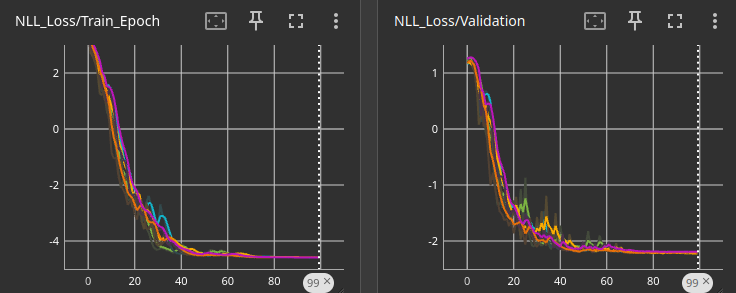
\includegraphics[width=\textwidth]{static/resnet/7-loss.png}
        \caption{Training and validation loss curves of the individual models of ensemble 7.}
        \label{fig:resnet-7-loss-curves}
    \end{subfigure}
    \begin{subfigure}{0.49\textwidth}
        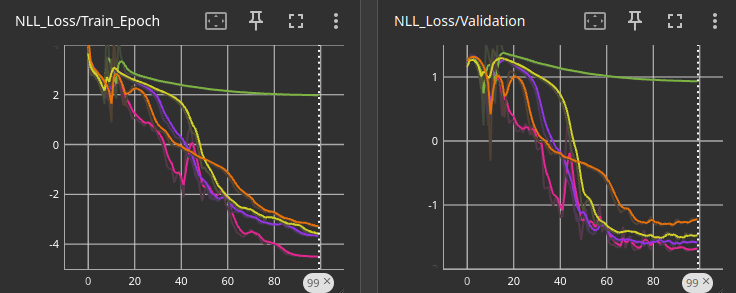
\includegraphics[width=\textwidth]{static/resnet/8-loss.png}
        \caption{Training and validation loss curves of the individual models of ensemble 8.}
        \label{fig:resnet-8-loss-curves}
    \end{subfigure}
    \caption{Training and validation loss curves of the individual models of the different ResNet ensembles.}
    \label{fig:resnet-loss-curves}
\end{figure}

One very obvious observation is the fact that the training of the ResNet models is very unstable.
Even a minor tweak in the architecture or the hyperparameters can lead to a very big difference in loss.
For example, when comparing models 1 and 4, which only differ a bit in learning rate, we can see a huge difference in validation loss of almost 4.
This is quite big when comparing the differences in the custom \gls{cnn} ensemble.

Also interesting to see is that increasing (or decreasing) the number of residual blocks does not necessarily lead to a better performance, as can be seen when comparing models 1, 2, and 3.
This can be explained by the pretrained weights, as they are trained on a classification task, and thus the later layers are more specialized for that task, failing to perform well on our regression task.
The first layers can be seen as feature extractors, which we need, while the later layers are optimized for the classification task, which we do not need.
Freezing the first layers is great, as the features to be extracted are not that different for the classification and regression task.
Freezing the later layers makes the model discard the spatial information, which is not needed for classification, but is needed for our regression task.

Other tweaks such as bagging, batch size, the number of models in the ensemble, etc. do not seem to have a significant effect on the performance of the model, as can be seen when comparing models 1, 5, 6, and 8.

Model 7, which does not use pretrained weights, performs surprisingly well, considering its size and the fact that it is trained from scratch on a small dataset.
When comparing its loss curves (\cref{fig:resnet-7-loss-curves}) with the other models, we can see that the individual models are more stable and converge faster.

We will keep models 6 and 7 for further comparison with the other models, as model 6 is smaller while still having a good performance, and model 7 is the best performing model.

\section{\gls{mc} dropout}\label{ch:models-for-uncertainty-aware-object-detection_section:mc-dropout}
\gls{mc} dropout, as explained in \cref{ch:literature-study_section:uncertainty-aware-ai-models_subsection:bayesian-neural-networks}, keeps dropout active during inference, creating an ensemble of models.
The architecture of the model used for \gls{mc} dropout is set up similarly to the simple \gls{cnn} described in \cref{ch:models-for-uncertainty-aware-object-detection_section:deep-ensembles_subsection:simple-cnn}, also enabling us to easily change the architecture of the model.
The main difference is, of course, the addition of dropout layers to the ``convolutional blocks''.
The dropout rate of each block can easily be changed so we can see the effect of different dropout rates on the performance of the model.

The training loop is a bit different from the one used for deep ensembles, as we only need to train a single model.
This model is trained like all the models in a deep ensemble, with the same loss function and the same way of feeding the training examples, adversarial training, etc.
There is the difference of having dropout available during training, so not using it would be a missed opportunity to regularize the model, so we keep it active during training as well.
The evaluating of the model after each epoch is also the same as for deep ensembles, we evaluate the model on the validation set and save and use the best model we get during training.
Note that dropout is disabled during validation so we can measure the model's true performance.

\paragraph{Comparing architectures and hyperparameter tuning}\label{ch:models-for-uncertainty-aware-object-detection_section:mc-dropout_comparing-architectures-and-hyperparameter-tuning}
\cref{tab:mc-dropout-architectures-comparison} and \cref{fig:mc-dropout-loss-curves} shows the results of some of the architectures we tested for the \gls{mc} dropout model as well as the hyperparameters.

\begin{table}[ht]
    \centering
    \begin{tabular}{c !{\vrule width 2pt} c|c|c|c|c|c !{\vrule width 2pt} c}
        \textbf{Index} & \textbf{Architecture} & \textbf{Dr} & \textbf{Lr} & \textbf{Bs} & \textbf{Epochs} & \textbf{F} & \textbf{Loss} \\
        \hline
        1 & [32, 64, 128] & 0.1 & $1\cdot10^{-4}$ & 32 & 100 & 100 & -2.0226 \\
        2 & [32, 64, 128] & 0.2 & $1\cdot10^{-4}$ & 32 & 100 & 100 & -1.6665 \\
        3 & [16, 32, 64] & 0.1 & $1\cdot10^{-4}$ & 32 & 100 & 100 & -1.9285 \\
        4 & [32, 64, 128] & 0.1 & $1\cdot10^{-4}$ & 16 & 100 & 100 & -2.1069 \\
        5 & [32, 64, 128] & 0.1 & $1\cdot10^{-3}$ & 32 & 100 & 100 & -1.9167 \\
        6 & [32, 64, 128] & 0.1 & $1\cdot10^{-4}$ & 32 & 100 & 1000 & -2.0246 \\
    \end{tabular}
    \caption[Comparison of different architectures for the \gls{mc} dropout model]{
        Comparison of different architectures for the \gls{mc} dropout model.
        ``Dr'' stands for dropout rate at each layer (we only experimented with the dropout rate staying constant over the layers), ``Lr'' stands for learning rate, ``Bs'' stands for batch size, ``Epochs'' stands for the number of epochs, ``F'' stands for the number of forward passes used in an ensemble, and ``Loss'' stands for the model's validation loss.
    }
    \label{tab:mc-dropout-architectures-comparison}
\end{table}

\begin{figure}[]
    \centering
    \begin{subfigure}{0.49\textwidth}
        
\includegraphics[width=\textwidth]{static/mc_dropout/1-loss.png}
        \caption{Training and validation loss curves of the MC dropout model with architecture 1.}
        \label{fig:mc-dropout-1-loss-curves}
    \end{subfigure}
    \begin{subfigure}{0.49\textwidth}
        
\includegraphics[width=\textwidth]{static/mc_dropout/2-loss.png}
        \caption{Training and validation loss curves of the MC dropout model with architecture 2.}
        \label{fig:mc-dropout-2-loss-curves}
    \end{subfigure}
    \begin{subfigure}{0.49\textwidth}
        
\includegraphics[width=\textwidth]{static/mc_dropout/3-loss.png}
        \caption{Training and validation loss curves of the MC dropout model with architecture 3.}
        \label{fig:mc-dropout-3-loss-curves}
    \end{subfigure}
    \begin{subfigure}{0.49\textwidth}
        
\includegraphics[width=\textwidth]{static/mc_dropout/4-loss.png}
        \caption{Training and validation loss curves of the MC dropout model with architecture 4.}
        \label{fig:mc-dropout-4-loss-curves}
    \end{subfigure}
    \begin{subfigure}{0.49\textwidth}
        
\includegraphics[width=\textwidth]{static/mc_dropout/5-loss.png}
        \caption{Training and validation loss curves of the MC dropout model with architecture 5.}
        \label{fig:mc-dropout-5-loss-curves}
    \end{subfigure}
    \begin{subfigure}{0.49\textwidth}
        
\includegraphics[width=\textwidth]{static/mc_dropout/6-loss.png}
        \caption{Training and validation loss curves of the MC dropout model with architecture 6.}
        \label{fig:mc-dropout-6-loss-curves}
    \end{subfigure}
    \caption{Training and validation loss curves of the different MC dropout models.}
    \label{fig:mc-dropout-loss-curves}
\end{figure}

The first thing which stands out when looking at the losses of the different models, is the fact that the dropout rate has a big effect on the performance.
When comparing models 1 and 2 for example, we can see that a higher dropout rate leads to a higher validation loss.
This is no big surprise, as each forward pass has only 80\% of the trained weights active, which obviously reduces the model's capabilities.

Interesting to see is that model 3, with a smaller architecture, performs roughly the same as model 1, which has a bigger architecture.
This can be interesting for faster inference times, as a smaller architecture will generally be faster than a bigger architecture.
This is already the case for a single forward pass, but it is even more the case for an ensemble of forward passes, as the number of forward passes is quite high.

When increasing the number of forward passes to 1000 (model 6), we do not see a significant drop in the validation loss compared to model 1, which only has 100 forward passes.
This means model 1 is well generalised, and increasing the number of forward passes does not bring a significant improvement.

The batch size and learning rate did not have that big of an effect on the performance (models 4 and 5).
The model with a higher learning rate (model 5) did however have a loss curve which is more unstable.

For the further experiments, we will use model 3 and 4.
Model 3 has a smaller architecture, which is interesting for faster inference times, and model 4 has the lowest validation loss.